\chapter{Spintronique moléculaire}

\section{Spintronique et Électronique moléculaire}
La microélectronique a su évoluer au gré des développements scientifiques. Elle a tout d'abord su tirer avantage des travaux sur la magnéto-résistance géante au travers d'une nouvelle discipline : la spintronique. Pendant presque deux décennies, celle-ci a permis d'améliorer de plusieurs ordres grandeurs les capacités de stockage des composants électroniques. Plus récemment, le développement de molécules organiques semi-conductrices~\cite{Tsumura1986,Horowitz1990,Lin1997} a poussé encore une fois l'électronique dans une nouvelle voie, celle de l'électronique moléculaire.

Ces deux évolutions pourraient bientôt se rejoindre afin de faire profiter du formidable potentiel des molécules modernes aux concepts issues de la spintronique

\subsection{La spintronique}
La spintronique est une branche de l'électronique où, en plus de la charge, le degré de liberté du spin est utilisé. Elle est notamment à l'origine des avancés technologiques les plus récentes telles que la MRAM~(Magnetic Random Access Memory) ou bien encore les têtes de lecture des disques durs. Mais le dispositif le plus célèbre, à la base des technologies précédemment citées, reste sans doute la vanne de spin. Celui-ci permet de filtrer les électrons en fonction de l'orientation de leur spin (soit \textit{up}, soit \textit{down}), autorisant un couplage direct entre magnétisme et courant électrique. La découverte du phénomène de magnétorésistance géante, à l'origine de ce filtrage, a d'ailleurs value à ces découvreurs, Albert Fert~\cite{Baibich1988} et Peter Grünberg~\cite{Gruenberg1986}, le prix Nobel de Physique en 2007.

\begin{figure}
\centering \includegraphics[scale=0.45]{Spintronique/SpinValve/SpinValve.pdf}
\caption{\textbf{a} : mesure de la résistance d'une valve de spin mettant en évidence la magnéto-résistance géante~(extrait de ~\cite{Baibich1988}).  \textbf{b} : Schéma d'une tête de lecture de disque dur dont le fonctionnement est basé sur le phénomène de magnéto-résistance~(extrait de Fujitsu).}
\label{SpinValve}
\end{figure}



La spintronique, dans ses applications, reste cependant cantonnée au stockage de  l'information~\cite{Awschalom2007}. Des propositions de spin-transistors directement commandés par le spin électronique ont pourtant été faites~\cite{Datta1990} et certains dispositifs ont également été réalisés~\cite{Johnson1996,Huang2007}. Mais de tels systèmes n'ont pas, pour l'instant, quitté les laboratoires.

Cependant, l'électron n'est pas la seule particule possédant spin, et des solutions de substitution peuvent être envisagées. Les aimants moléculaires sont des candidats sérieux~\cite{Bogani2008}. Du fait des développements récents de l'électronique moléculaire, ils pourraient bientôt faire partie intégrante des dispositifs électroniques.

\subsection{L'électronique moléculaire}
Devant le besoin toujours plus grand de miniaturisation des dispositifs, les chercheurs et les industriels se sont vite rendu compte des limites des techniques de fabrication traditionnelles. Elles consistent à partir d'un matériaux massif et de graver en son sein, les structures nanométriques nécessaires à la production de l'électronique actuelle.

Devant le progrès récent de la chimie organique, une seconde solution est apparue, faisant appel à cette dernière  pour produire les objets de petite taille et les disposer de manière contrôlée, afin de produire des composants électroniques : c'est l'approche ``Bottom-Up". L'histoire de l'électronique moléculaire est cependant relativement récente. Comme le rappelle G. Horowitz dans~\cite{Klauk2007} , l'industrie s'est finalement intéressée à ce domaine de l'électronique lorsque les semi-conducteurs organiques sont devenus plus performants, en terme de mobilité des électrons, que le silicium amorphe~\cite{Lin1997}.
\begin{figure}
\centering \includegraphics[scale=0.45]{Spintronique/MolecularElec/MolecularElec.pdf}
\caption{\textbf{a} : Photographie d'un substrat de polymide contenant des transistor organique. \textbf{b} : Vue en coupe d'un transistor organique~(figure extraite de~\cite{Sekitani2010}).}
\label{MolecularElec}
\end{figure}


Depuis, de nombreux dispositifs issus de l'électronique moléculaire ont vu le jour, comme les  transistors à base de films fins organiques (ou OFTFs). Mais aucune application n'a, à ce jour, tiré partie de la petite taille des molécules, et la route est encore longue avant l'obtention de dispositifs commerciaux ne mettant en jeux que quelques molécules, voire une seule.

Comme le rappelle les auteurs de~\cite{Gatteschi2006} , une conséquence un plus inattendu du développement de l'électronique moléculaire est d'avoir participé à l'essor du magnétisme moléculaire, domaine que nous allons aborder maintenant.


\section{Le magnétisme moléculaire}
Essayer de dresser un panel complet du magnétisme moléculaire est un travail complexe auquel je ne m'attacherai pas ici. Pour cela, je renvois le lecteur à~\cite{Gatteschi2006} et son excellente introduction. Je ne vais souligner ici que quelques étapes présentant certains des phénomènes physiques majeurs mis en évidence dans les aimants moléculaires.

\begin{figure}
\centering \includegraphics[scale=0.45]{Spintronique/MolecularMag/MolecularMag.pdf}
\caption{\textbf{a} : Première mesure du phénomène de QTM sur un cristal moléculaire de Mn$_{12}$Ac~(extrait de~\cite{Thomas1996}). \textbf{b} : Mise en évidence du phénomène d'interférence relatif au retournement de l'aimantation d'un cristal moléculaire de Fe$_{8}$~(extrait de~\cite{Wernsdorfer1999}).}
\label{MolecularMag}
\end{figure}

La première mesure d'un effet quantique sur un aimant moléculaire~(~SMM ou Single Molecular Magnet) a été obtenue en 1995 à partir d'un échantillon de poudre de SMMs~\cite{Friedman1996}. Un an plus tard, cette mesure était confirmée à l'aide d'un cristal composé d'un SMM bien connu : le Mn$_{12}$Ac~\cite{Thomas1996}. Cet effet quantique est connu sous le nom de retournement de l'aimantation par effet tunnel~(ou QTM - Quantum Tunneling of the Magnetization).

Celui-ci correspond au retournement de l'aimantation d'une molécule malgré la présence d'une barrière de potentiel entre les deux orientations opposées. Tout ce passe comme si l'aimantation passait à travers cette barrière par effet tunnel, d'où le nom. Ceci n'est possible que lorsque deux états du système, situés de part et d'autre du puits de potentiel, sont amenés en résonance à l'aide d'un champ magnétique. Le phénomène de QTM ne peut se faire que pour des valeurs de champ magnétique bien précises donnant lieux à des mesure de cycle d'hystérésis présentant des marches. L'annexe concernant les aimants moléculaires traite en détail de ce phénomène.

Trois ans plus tard, Wolfgang Wernsdorfer et Roberta Sessoli mettaient en évidence l'oscillation des \textit{splitings} tunnels dû à un effet quantique d'interférence semblable à la phase de Berry~\cite{Wernsdorfer1999}. Dans ce phénomène, les interférences se font entre le différents ``chemins" que l’aimantation peut prendre sur la sphère de Bloch lors de son renversement. Ceci se traduit par une variation dans les probabilités de retournement et donc, par une modulation de la hauteur des marches associés au QTM.

La structure hyperfine de certains noyaux parmis les terres rares, ont pu également être exploré. En effet, la position en champ des retournement par QTM peut être, dans certains cas, fortement influencé par l'état du spin nucléaire. Le TbPc$_{2}$, où Terbium Double-Decker~( en référence aux avions à deux ailes), a notamment été caractérisé en détail à l'aide de la technique microSQUID, et les paramètres de couplage hyperfin ont pu être extraits de la mesure de l'aimantation d'un cristal moléculaire. D'autre noyaux que le Tb ont également été analysés avec succès à l'aide d'une structure moléculaire identique.

\begin{figure}
\centering \includegraphics[scale=0.45]{Spintronique/MolecularMag2/MolecularMag2.pdf}
\caption{\textbf{a} : Structure du \textit{cluster} de Fe$_4$. \textbf{b} : Représentation des différent mode d'ancrage~(extrait de ??).}
\label{MolecularMag2}
\end{figure}

Mais les progrès de l'électronique moléculaire n'ont pas laissé la communauté du magnétisme indifférente et la question de l'interaction entre aimant moléculaire et surface métallique à commencé à se poser. Une étude portant sur une molécule de Mn$_{12}$ déposé sur une surface d'or a été réalisée en 2008 en combinant différents moyen d'analyse~(XAS et XMCD). Elle conclue que la structure de l'aimant moléculaire est modifiée lorsque ce dernier est déposé sur une surface et que le magnétisme est également affecté.[voir ref 11 et 12 Sessoli]Cette fragilité des aimants moléculaire a été confirmé par une seconde série de mesure soulignant l'importance du choix du SMM pour les application de spintronique moléculaire.

%De nombreuses expériences ont suivi permettant de jeter la lumière sur de nouveaux aimants moléculaires. Les techniques expérimentales ont également beaucoup évolué avec le développement de la spintronique moléculaire. A l'aide de cette dernière, des mesures sur un aimant moléculaire unique mettant en évidence le phénomène de QTM ont été menés à l'aide d'une valve de spin à base de nanotube de carbonne et de TbPc$_{2}$.

Une meilleure compréhension du magnétisme moléculaire et ses interactions avec l’environnement passe par le développement de la spintronique moléculaire, seul moyen d'investigation à l'échelle de la molécule unique. C'est donc également dans cette voie que se sont engagé à la fois les chimiste et les physiciens comme nous allons le voir maintenant.


\section{La spintronique moléculaire}
La spintronique moléculaire a pour but de combiner les techniques de la spintronique avec les nouveaux développements de l'électronique moléculaire et de la chimie, afin de produire de nouveaux dispositif susceptible de compléter ou éventuellement remplacer les technologies tout semi-conducteurs déjà existantes. Cette discipline a connue une évolution rapide ces dernières années, bénéficiant des dernières avancés en matière de lithographie, mais aussi de la mise en synergie du travail des physiciens et des chimistes. 

Dans ce paragraphe, je ne présenterai bien sûr qu'une petite partie des nombreux travaux effectués dans le domaine. Ceci ne constitue donc en aucun cas une liste exhaustive des expériences réalisées, ni m\^eme une sélection des travaux les plus importants. Elle permettrons néanmoins, je l'espère, d'aider le lecteur à situer nos recherche par rapport à celles en cours dans d'autres laboratoires. De plus, je me limiterai ici aux dispositifs ne comportant qu'un nombre limités de molécules, de l'ordre de l'unité, généralement utilisés dans les laboratoires de recherche fondamentale.
\subsection{État de l'art}

\subsubsection*{Du premier transistor moléculaire...}
La première expérience de mesure de courant à travers une molécule unique a été faite en 1995 à l'aide un microscope à effet tunnel~( ou STM). Il s'agissait de mesurer la résistance à travers une molécule de C$_{60}$ déposée sur une surface d'or. Il n'était pas question d'obtenir un transistor, puisque seul deux terminaux étaient présents à savoir, la surface conductrice et la pointe du STM.

Cette expérience, et celles qui ont suivi, ont encouragé le développement de nouvelles techniques permettant de piéger une molécule unique dans un dispositif de mesure. C'est ainsi qu'est apparu la technique dite de "break junction". Elle consiste à suspendre un fin pont métallique puis à plier le support jusqu'à obtenir une cassure. La taille de celle-ci peut être ensuite modulée en faisant varier la courbure imposée à l'échantillon. A l'aide de ce dispositif, Reed et ses collègues ont pu mesurer, en 1997, des molécules de benzene-1,4-dithiol et montrer l'influence du couplage entre les électrodes et la molécule, sur la conductance mesurée. Cette technique présente cependant l'inconvénient de ne pas pouvoir disposer d'une grille permettant de moduler le potentiel de la molécule.

\begin{figure}
\centering 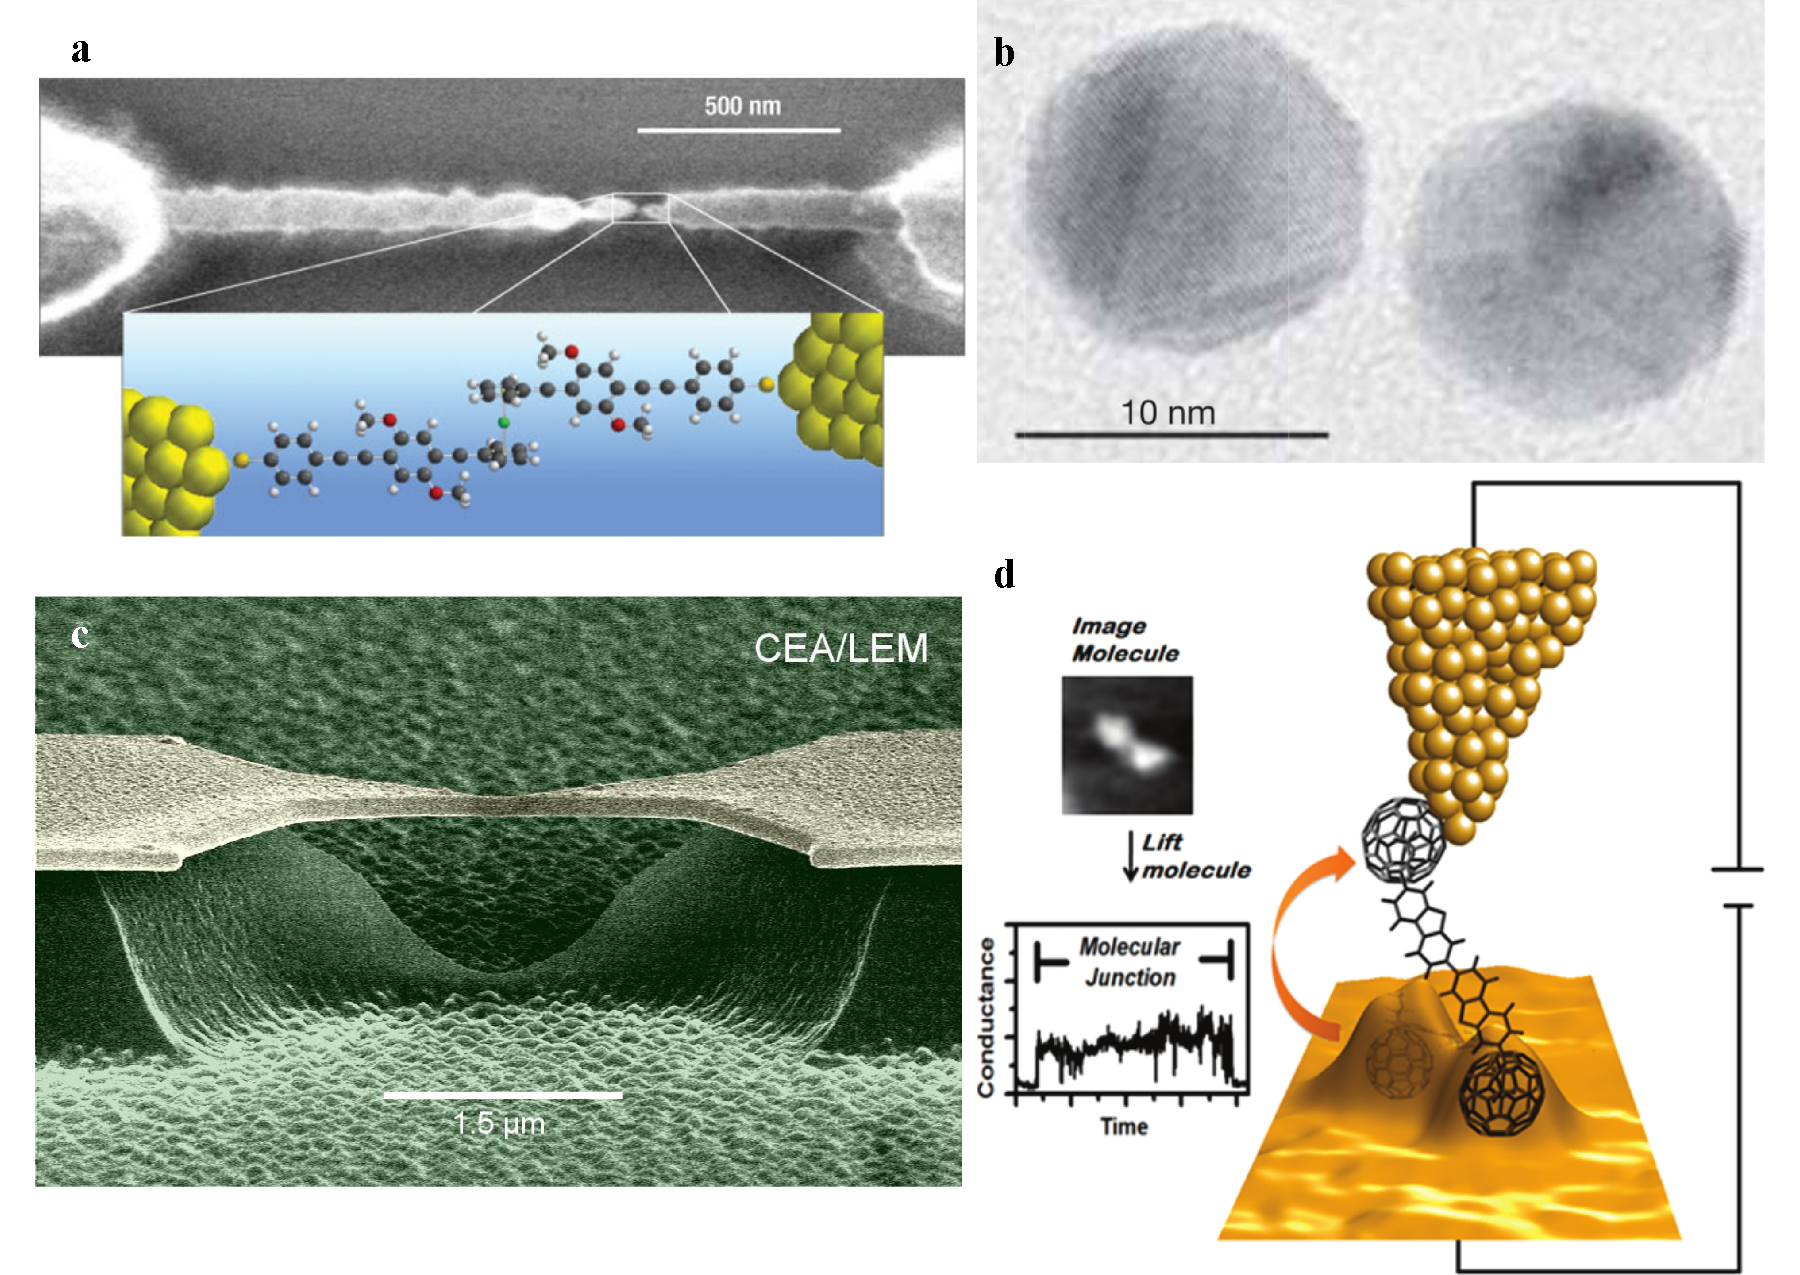
\includegraphics[scale=0.45]{Spintronique/MolSpintro2/MolSpintro2.pdf}
\caption{\textbf{a} : Structure de trois molecules : 1,4-benzenedimethanethiol~(BDMT), 4,4'-biphenyldithiol~(BPD) et bis-(4-mercaptophenyl)-ether~(BPE). \textbf{b} : Mécanisme de prise de contact. \textbf{c-e} : Image par microscopie électronique à transmission~(TEM) des structure de dimer, trimer et tetramer composé de bille d'or de $50\,nm$. \textbf{f} : image TEM d'un dimer à base de BDMT constitué par deux billes d'or de $10\,nm$. Le nanomètre qui sépare les deux billes correspond approximativement à la taille de la molécule de BDMT~($0.9\,nm$).Figure extraite de ??}
\label{MolSpintro2}
\end{figure}


Pour pallier à cet inconvénient, il a fallu attendre encore 3 ans et la réalisation du premier transistor à molécule unique. Celui-ci consistait en un atome de C$_{60}$ piégé entre deux électrodes d'or et une grille. Ce dispositif a été obtenue en faisant circuler une forte densité de courant dans un fil fin d'or, venant provoquer la migration des atomes au niveau du point faible et provocant une cassure de l'ordre du nanomètre. Le phénomène d'électromigration est un phénomène bien connu des micro-électroniciens puisqu'il est à l'origine de certaines défaillance dans les puces et autres dispositifs électroniques. Il a d'ailleurs donné son nom à la technique : l'électromigration. Nous présenterons cette dernière plus en détail dans le chapitre consacré à la fabrication de notre échantillon. L'expérience menée sur ce premier transistor moléculaire avait pu mettre en évidence le couplage entre les vibrations moléculaires et la résistance du dispositif. De plus, la grille se révélait suffisamment efficace pour modifier l'état de charge de la molécule de C$_{60}$ permettant ainsi d'obtenir les premiers diamants de Coulomb associé à une molécule unique.

Une étape supplémentaire a été franchi par le groupe de A. Yacoby. Ils ont mis au point la première approche réellement ``Bottom-Up" en attachant chimiquement une molécule à deux bille d'or de quelques nanomètre, pour venir ensuite contacter ces dernières à l'aide de deux électrodes. Cependant, à ma connaissance, cette technique n'a pas été réutilisée. Elle illustre néanmoins les nombreuses possibilités qu'offre la fonctionnalisation.

Cependant, dans ces dispositifs, aucune propriété propre aux molécules n'est utilisée et le seul spin en jeu dans les phénomènes observés reste celui de l'électron. Hors, l'avantage principal des molécules, outre leur taille, provient des différentes propriétés, notamment magnétique, que la chimie moderne peut leur conférer.

\subsubsection*{\`A la spintronique moléculaire}

L'année 2006 a vu paraître les deux premières expériences visant à insérer des aimants moléculaires au sein d'un gap afin d'obtenir les premiers dispositifs de spintronique moléculaire. La première a été publiée par le groupe de H.S.J van der Zant et la seconde par le groupe de D.C. Ralph, et portaient toutes deux sur l'étude d'un aimant moléculaire bien connu : le Mn$_{12}$. Un des aspects intéressant de ces expériences, outre le magnétisme de la molécule, est la fonctionnalisation de cette dernière à l'aide de groupe thiol, afin de favoriser le couplage avec les électrodes d'or. En effet, il illustre la souplesse de la chimie de part la possibilité qu'elle offre de fabriquer des molécules faites sur mesure, afin de faciliter certaines configurations ou certains comportements~(ici une forte affinité avec l'or).  

Cependant, les mesures en transport, bien que montrant une dépendance en champ magnétique complexe et des signes de conductance différentielle négative, n'ont pas permis de confirmer, de façon certaine, s'il s'agissait bien d'une molécule de Mn$_{12}$, ni même de savoir si les propriétés magnétiques de cette dernière avait été conservées durant la fabrication. Le groupe de D.C. Ralph conclue d'ailleurs ses travaux par la phrase suivante : ``We find significant variations between devices, indicating that the sample fabrication process and the device environment may affect our molecules".

La première expérience réellement convaincante de transistors moléculaires mettant en jeu une molécule magnétique a été réalisée en 2008 dans le groupe de D.C. Ralph. Toujours avec la technique d'électromigration, son équipe avait produit un transistor à base de N@C$_{60}$. Elle avait alors pu mettre en évidence, à travers de mesure en transport, le magnétisme lié à l'atome d'azote de spin S=3/2,  et remonter au couplage entre ce dernier et les électrons de la cage de C$_{60}$. 

\begin{figure}
\centering \includegraphics[scale=0.45]{Spintronique/MolSpintro/MolSpintro.pdf}
\caption{\textbf{a} : Structure du Mn$_{12}$ entouré de ligands thiols favorisant l'ancrage. \textbf{b} : Représentation schématique de la molécule de Mn$_{12}$ piégée entre les électrodes. \textbf{c} : Image de la jonctions obtenue par microscopie électronique. Le trait blanc correspond à $200\,nm$.~(extrait de ??).}
\label{MolSpintro}
\end{figure}

Il s'agit, à mes yeux, du premier dispositif que l'on peut qualifier de spintronique moléculaire à l'échelle de la molécule unique. En effet, les propriétés magnétiques de la molécule isolée se retrouvent de façon non-équivoque dans les mesures en transport. Ce n'est d'ailleurs pas surprenant car, fort de leur expérience avec le Mn$_{12}$, les auteurs avaient choisi le N@C$_{60}$ pour la robustesse de sa structure et de ses propriétés magnétiques, comme ils le précisent dans leur papier. Cependant, bien que possédant un moment magnétique, cette dernière n'appartient pas à la catégorie des aimants moléculaires. En effet, elle ne possède pas d'axe facile et l'orientation de son moment magnétique n'est déterminé que par le champ magnétique. Il est donc impossible d'observer dans cette molécule, les phénomènes quantiques présentés dans le cadre du magnétisme moléculaire.

Loin d'\^etre des échecs, ces différents travaux ont fournis un apport important au reste de la communauté notamment concernant les critères essentiels que doivent remplir les aimants moléculaires susceptibles d'être étudiés par les techniques expérimentales actuelles. Je détaillerai ces différents critères lorsque j'introduirai le Terbium double-Decker.
 
\subsection{La spintronique dans notre groupe}
Le groupe au sein duquel j'ai effectué ma thèse a une culture ancrée dans le nano-magnétisme et le magnétisme moléculaire. Une bonne partie des efforts de la fin des année 1990 et du début des années 2000 a été consacré à l'analyse et la caractérisation de systèmes magnétiques allant de la nanoparticule au cristal moléculaire  et plus récemment, l'aimant moléculaire isolé et le spin nucléaire unique. A chaque échelle de mesure correspond un appareil de mesure, et assez logiquement, plus le système à mesurer est petit, plus le détecteur l'est. Cette tendance est bien représentée dans la figure ??. Pour des particules macroscopiques, l'usage d'un SQUID est suffisant. Lorsque l'on veut caractérisé des particules de l'ordre de quelques dizaines de nanomètre ou bien encore un cristal moléculaire, l'usage d'un détecteur aussi sensible qu'un microSQUID est indispensable.

Lorsque l'objet a détecter devient très petit, comme une molécule par exemple, il n'est plus vraiment possible de faire la distinction entre le détecteur et l'objet à mesurer. Il faut alors songer à fabriquer un dispositif électronique dont le fonctionnement même est influencé par le magnétisme de l'un de ses composants. Autrement dit, il faut faire appel à la spintronique et plus précisément, lorsque l'on s'intéresse aux molécules, à la spintronique moléculaire.

C'est dans ce cadre que se sont effectué les premiers travaux conduisant à la fabrication du premier nanosquid en 2006. Celui-ci,  composé de deux liens faible supraconducteur à base de nanotube, a permis de mesurer, en transport, une astroide de StonerWolfarth, mesure caractéristique des propriétés magnétiques d'une nanoparticule. Ces nanoparticules avait pour particularité d'être inséré dans les Nanotube plutôt que déposé sur le dispositif, faisant parti intégrante du système.

Parallèlement aux travaux sur le nanoSQUID, notre groupe a développé, à partir des travaux de H. Park, sa propre technique d'électromigration basée sur une boucle de contre réaction rapide. Ces travaux ont d'abord permis la réalisation d'un transistor moléculaire à base de C$_{60}$. Celui-ci à conduit à l'observation de nombreux phénomènes quantiques tels que l'effet Kondo sous-écranté ou bien encore la transition de phase quantique. Puis, en collaboration avec W. Harneit, nous avons étudié la molécule de N@C$_{60}$, confirmant les résultats obtenus quelques temps plus tôt par D.C. Raplh et complétant ses observations par des mesures en cotunneling. L'ensemble de ces travaux peut être trouvé dans la thèse de Nicolas Roch.

Cette première analyse d'une molécule magnétique nous a également permis d'identifier les faiblesses de notre dispositif expérimental. Il nous fallait ajouter deux axes magnétiques pour explorer les trois directions de l'espace, mais également être capable de balayer le champ beaucoup plus rapidement : avec des vitesse de plusieurs centaines de milli-Tesla par seconde. Fort de l'expérience du groupe dans le domaine du nanomagnétisme, un dispositif mettant en jeux deux bobines de faible inductance et un système de dilution rotative a été développé rapidement au sein du laboratoire. Ce dispositif a permis d'obtenir les résultats que je vais vous présenter dans cette thèse.

La thématique des nanotubes n'est cepedant pas restée inactive, de nouveaux dispositifs ont été développés et ont donné des résultats encourageants. C'est notamment le cas de la vanne de spin obtenue par Matias Urdampilleta. Dans son expérience, un tube a été relié à deux électrodes, une grille permettant de faire varier son potentiel. Un solution contenant des molécules de TbPc$_{2}$ a ensuite été déposée, puis l'échantillon a été disposé dans un frigo à dilution. Les résultats ont mis en évidence un comportement de type vanne de spin et une analyse fine des mesures a permis de déterminer que les rôles de polariseur et d'analyseur étaient joués par deux aimants moléculaires. Ces travaux ont bien sûr fait l'objet d'un publication. Il s'agit là du premier dispositif de spintronique moléculaire mettant en jeux des aimants moléculaires. Il est assez amusant de constater que le premier dispositif qui a permis de mettre la spintronique sur le devant de la scène soit également la premier a être réalisé en spintronique moléculaire.